% Preambulo
\documentclass[12pt,a4paper]{report}
\usepackage[utf8]{inputenc}
\usepackage[portuges]{babel}
\usepackage{a4wide}
\usepackage{graphicx}
\graphicspath{ {images/} }
\usepackage[myheadings]{fullpage}
\usepackage[shortlabels]{enumitem}
\usepackage{indentfirst} %Faz automáticamente os parágrafos.
\usepackage{color}
\usepackage[dvipsnames]{xcolor}
\usepackage{minted}
\usepackage[export]{adjustbox}
\usepackage{subcaption}

\setcounter{secnumdepth}{5}
\captionsetup[figure]{
         labelfont={small},
         font={small}
         }

\usemintedstyle{friendly}
\definecolor{bg}{rgb}{0.90,0.90,0.90}
\newcommand{\HRule}[1]{\rule{\linewidth}{#1}}

\begin{document}

%Capa do Relatório
\begin{titlepage}
    \centering
    \begin{figure}[h]
    
\includegraphics[scale=2]{images/logo_um_eng.jpg}
    \centering
    \end{figure}
    {\scshape\huge\bfseries {Universidade do Minho}\par}
    \vspace{0.5cm}
    {\scshape\large{Mestrado Integrado em Engenharia Informártica}\par}
    \vspace{6cm}
    %\HRule{1pt} \\
    %{\Huge\bfseries\textcolor{Cyan}{SOKOBAN} \par}
    %\HRule{2pt} \\ [0.7cm]
    \begin{figure}[h]
    
\includegraphics[scale=11]{images/logo.png}
    \centering
    \end{figure}
    {\Large\bfseries Laboratórios de Informática I\par}
    \vspace{4cm}
    {\scshape\Large Grupo li1g126\par}
    \vspace{1cm}
    {\Large\itshape Miguel Magalhães (a77789)\par}
    {\Large\itshape Hugo Oliveira (a78565)\par}
    \vfill
    {\large \today\par}
\end{titlepage}

%Índice
\tableofcontents
\thispagestyle{empty}
\newpage

%Resumo
\begin{abstract}

Este documento, desenvolvido na unidade curricular de Laboratórios de Informática 1 (LI1), apresenta uma resolução de um jogo do tipo Sokoban.\\

Um dos objetivos da resolução deste problema, é tornar o jogo diferente do típico jogo Sokoban, como tal, foi acrescentado ao jogo a possibilidade de alterar o tema, de alterar os níveis de jogo, de utilizar Undo e Restart ainda de poder visualizar o Score.\\

O relatório baseia-se, fundamentalmente, nas partes mais importantes dos códigos desenvolvidos na resolução do jogo.
Assim, este está dividido em 4 partes, sendo que as duas últimas são as mais importantes: Fase Inicial do jogo, Solver, Movimentação do Sokoban e ainda Interface Gráfica.

\end{abstract}


%Introdução
\chapter{Introdução}
\label{sec:intro}


Ao longo deste trabalho iremos explicar alguns dos passos fundamentais à realização do jogo \emph{Sokoban}. Com isso pretendemos fazer um percurso objetivo e rigoroso sobre a resolução deste problema. 

Todo o jogo foi desenvolvido na linguagem de programação funcional Haskell. É de notar, que neste relatório, nos incidimos sobretudo na realização da última tarefa, que consiste na realização da interface gráfica do jogo, onde recorremos à biblioteca \emph{Gloss}.


%Esta secção termina normalmente com uma apresentação da estrutura do relatório, sendo aqui apresentada uma sugestão. Neste caso, a Secção~\ref{sec:problema} descreve o problema a resolver enquanto a Secção~\ref{sec:solucao} apresenta e discute a solução proposta pelos alunos. O relatório termina com conclusões na Secção~\ref{sec:conclusao}, onde é também apresentada uma análise crítica dos resultados obtidos.


\chapter{Descrição do Problema}
\label{sec:problema}

A realização do jogo tem por base a leitura do \textbf{mapa}, da \textbf{posição do boneco} e ainda das \textbf{coordenadas das caixas}. Todos estes dados contribuem para realização do jogo. Como tal, o \textbf{input} (mapa, posição do boneco e coordenadas das caixas) tem de obedecer a determinadas regras, tais como:

\begin{itemize}
  \item Todos os mapas de jogo têm de ter sempre uma estrutura retangular; 
  \item '\#' representa uma parede;
  \item '\space' representa uma área livre;
  \item '.' representa um local de arrumação;
  \item logo após o mapa, as primeiras coordenadas representam a posição do boneco;
  \item as restantes coordenadas representam as posições das caixas;
  \item todas estas coordenadas não se podem sobrepor entre si nem se sobrepor com o mapa (tabuleiro).
\end{itemize}


Após a verificação de todas estas regras é necessário animar o \emph{Sokoban}, partindo de movimentações nos eixos \emph{x} e \emph{y} para: cima, baixo, esquerda e direita. 

Primeiramente, é analizada jogoda a jogada a possibilidade de movimentação no mapa e as suas consequências nos objetos para além do jogogador, nomeadamente na movimentação das caixas.

Por conseguinte, todo o jogo é convertido para uma \emph{interface gráfica}, permitindo assim, o utilizador jogar. Nesta parte da tarefa, recorremos à biblioteca \emph{Gloss}.


%temas\thanks{Sokoban, Lego, Lager , entre outros.}

\newpage
\chapter{Concepção da Solução}
\section{Estruturas de Dados}

Para podermos organizar da melhor forma o código, definimos alguns tipos, facilitando a tanto a escrita como a leitura.

\begin{itemize}
  \item \textbf{type Input          = [String]}   - lista com todos os dados necessários;    
  \item \textbf{type Tabuleiro      = [String]}   - lista com o mapa em si;
  \item \textbf{type NivelMapa      = String}     - tabuleiro numa string apenas;
  \item \textbf{type Coords         = [String]}   - lista de coordenadas;
  \item \textbf{type Posicao        = (Int,Int)}  - coordenada (x,y);
  \item \textbf{type TickCount      = Int}        - número de movimentos;
  \item \textbf{type Comandos       = String}     - string com os comandos, ex: "ULRD" ;
  \item \textbf{type Linha          = String}     - linha do tabuleiro;
  \item \textbf{type ComandoSimples = Char}       - um comando, ex: 'U';
  \item \textbf{type Bitmaps        = [Picture]}  - lista com todos os bitmaps necessários para desenhar o mapa e aprensentar ao jogador;
  \item \textbf{type Bomba          = Bool}       - existência de uma bomba ou não;
  \item \textbf{type Contador       = Float}      - contador do tipo Float;
  \item \textbf{type Level          = String}     - numero de um nível ex: "3";
  \item \textbf{type Tema           = String}     - nome de um tema ex: "Lego";
  \item \textbf{type Highscore      = String}     - melhor pontuação obtida ex: "324";
  \item \textbf{type Mapa = (Bitmaps,NivelMapa,Comandos,Bomba)} - base do jogo.
\end{itemize}


\section{Implementação}
\subsection{Fase Inicial}

 \hfill

Na fase inicial de jogo foi necessário perceber quais eram os \emph{inputs} válidos. Estes inputs numa primeira abordagem consistiam apenas num mapa seguido de coordanadas, das quais a primeira seria a posição do boneco e as restantes as posições das caixas.

O jogador irá recorrer às teclas 'W', 'A', 'S' e 'D' para mover o Sokoban.
Consequentemente, para melhor perceber o mecanismo de jogo, começamos por desenvolver um código com base na \textbf{Tarefa4}. Este código, permitiu a visualizaçãp no terminal da movimentação do Sokoban. Isto é, após o jogador premir uma tecla de jogo, é possível ver a posição final do Sokoban depois de este comando ser executado.\\

\begin{figure}[htb]
\centering
  \begin{tabular}{@{}cc@{}}
    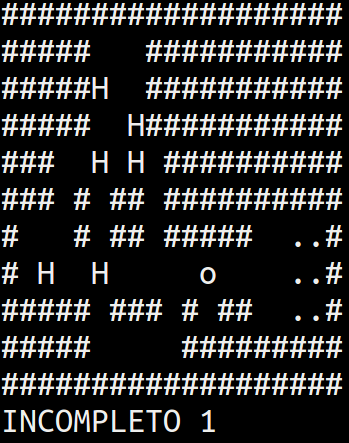
\includegraphics[scale=0.42]{images/Capturar1.PNG} &
    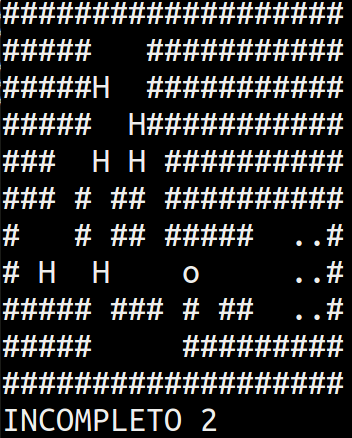
\includegraphics[scale=0.42]{images/Capturar2.PNG}
  \end{tabular}
  \caption{Após premir W e A respetivamente}
\end{figure}

\hfill

Para que fosse possível adicionar os comandos 'U', 'L', 'D' e 'R' no \emph{input} criámos um programa que permite interagir com ficheiro \emph{tab1.in} (mapa de teste) e com uma adaptação da tarefa 4 que resulta num jogo interativo no terminal.

\hfill

\begin{minted}[bgcolor=bg, 
               fontsize=\footnotesize, 
               framesep=2mm,
               linenos,
               breaklines,
               breakautoindent=true,
               breaksymbolleft=\raisebox{0.8ex}{\tiny\hookrightarrow},
               breaksymbolindentleft=0pt,
               breaksymbolsepleft=1pt,
               breaksymbolright=\raisebox{0.8ex}{\tiny\hookleftarrow},
               breaksymbolindentright=0pt,
               breaksymbolsepright=1pt
]{haskell}
main = do
  hSetEcho stdin False
  hSetBuffering stdin NoBuffering
  c <- getChar
  if c == 'q'
    then do return ()
    else do addcmd c
            hSetEcho stdin True
            callCommand "clear"
            callCommand "./tarefa4_modified < tab1.in"
            main
   where addcmd c
           | c == 'w' || c =='W' = appendFile "tab1.in" "U"
           | c == 'a' || c =='A' = appendFile "tab1.in" "L"
           | c == 's' || c =='S' = appendFile "tab1.in" "D"
           | c == 'd' || c =='D' = appendFile "tab1.in" "R"
           | otherwise           = appendFile "tab1.in" ""
\end{minted}

\subsection{Solver}

Numa tentativa de aplicar no jogo a funcionalidade do jogador obter uma resolução de um certo nível, foi desenvolvida o programa \emph{solver}.

Para isso é gerada uma série de soluções por ordem crescente de tamanho. São testadas todas as combinações possíveis até que seja encontrada a solução do nível. Como as soluções testadas por ordem de crescente de tamanho, sempre que é encontrada uma solução é garantido que esta é a melhor solução para o mapa que está a ser testado.\\

A função \emph{comands} gera os comandos que são posteriormente testados pela \emph{trySolution} que vai testando os comandos gerados até encontrar a solução.

\begin{minted}[bgcolor=bg, 
               fontsize=\footnotesize, 
               framesep=2mm,
               linenos,
               breaklines,
               breakautoindent=true,
               breaksymbolleft=\raisebox{0.8ex}{\tiny\hookrightarrow},
               breaksymbolindentleft=0pt,
               breaksymbolsepleft=1pt,
               breaksymbolright=\raisebox{0.8ex}{\tiny\hookleftarrow},
               breaksymbolindentright=0pt,
               breaksymbolsepright=1pt
]{haskell}

trySolution tab n
  | jogada tab (comands !! n) == "1" = (comands !! n)
  | otherwise = trySolution tab (n+1)

\end{minted}

\begin{minted}[bgcolor=bg, 
               fontsize=\footnotesize, 
               framesep=2mm,
               linenos,
               breaklines,
               breakautoindent=true,
               breaksymbolleft=\raisebox{0.8ex}{\tiny\hookrightarrow},
               breaksymbolindentleft=0pt,
               breaksymbolsepleft=1pt,
               breaksymbolright=\raisebox{0.8ex}{\tiny\hookleftarrow},
               breaksymbolindentright=0pt,
               breaksymbolsepright=1pt
]{haskell}

comands = [0..] >>= flip replicateM "URLD"

\end{minted}

\hfill

\hfill

Dado que para níveis de elevada complexidade a função leva demasiado tempo a encontrar uma solução, esta mesma funcionalidade não foi adicionada ao jogo. Isto por ser um solver por \emph{brute force}. No entanto, encontra-se em baixo um exemplo para um tabuleiro de pouca complexidade.

\hfill

\begin{figure}[h]
    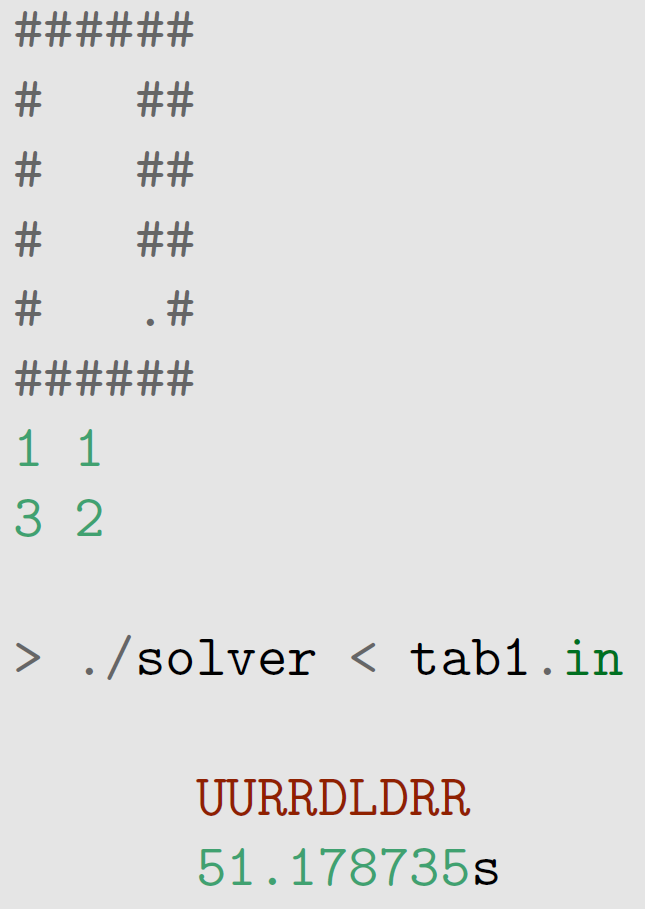
\includegraphics[scale=0.3]{images/Capturar3.PNG}
    \centering
    \caption{Exemplo de execução da função Solver}
\end{figure}


\newpage

\subsection{Movimentação do Sokoban}

\hfill


Adaptámos a \textbf{Tarefa4} de modo a funcionar como um "esqueleto do jogo". Todo este código diz respeito à movimentação do Sokoban.

A função \emph{checkMov} exibe o tabuleiro de jogo após todas as movimentações e as implicações destas movimentações terem sido realizadas. 
 
\hfill

\begin{minted}[bgcolor=bg, 
               fontsize=\footnotesize, 
               framesep=2mm,
               linenos,
               breaklines,
               breakautoindent=true,
               breaksymbolleft=\raisebox{0.8ex}{\tiny\hookrightarrow},
               breaksymbolindentleft=0pt,
               breaksymbolsepleft=1pt,
               breaksymbolright=\raisebox{0.8ex}{\tiny\hookleftarrow},
               breaksymbolindentright=0pt,
               breaksymbolsepright=1pt
]{haskell}

checkMov :: Tabuleiro -> TickCount -> Comandos -> Posicao -> Tabuleiro
checkMov l p c b
    | existemH tabCBoneco == 0  = tabCBoneco ++ ["FIM " ++ show p]
    | null c  = tabCBoneco ++ ["INCOMPLETO " ++ show p]
    | b == move l b [head c] && [head c] /= "B" = checkMov l p (tail c) b
    | otherwise  = checkMov movimentacao (p+1) (tail c) (move l b [head c])
    where tabCBoneco  = colocCaixas (rmBoneco l) [b] 1
          movimentacao = if [head c] == "B"
                          then bomba l b
                          else (mvBoxAux tabCBoneco b [(head c)])
\end{minted}

\hfill

\hfill

Quando é efetuado um movimento, o Sokoban pode alterar de posição ou então permanecer no mesmo local.
Para isso, é necessário saber, tendo em conta a posição do Sokoban e a direção para onde se vai mover, qual irá ser o obstáculo que irá encontrar e de que forma proceder de acordo com essa análise.

Foi desenvolvida a seguinta função que permite, para qualquer \textbf{movimento}, testar a posição final do Sokoban e, desse modo, fornecer essa mesma posição. (Segue-se um exemplo para o caso de o moviemento ser \emph{Up}, para os restantes é análogo.)\\


\begin{minted}[bgcolor=bg, 
               fontsize=\footnotesize, 
               framesep=2mm,
               linenos,
               breaklines,
               breakautoindent=true,
               breaksymbolleft=\raisebox{0.8ex}{\tiny\hookrightarrow},
               breaksymbolindentleft=0pt,
               breaksymbolsepleft=1pt,
               breaksymbolright=\raisebox{0.8ex}{\tiny\hookleftarrow},
               breaksymbolindentright=0pt,
               breaksymbolsepright=1pt
]{haskell}

move :: Tabuleiro -> Posicao -> Movimento -> Posicao
move tab (a,b) "U"
    | up == '#' || (elem up "IH" && elem up2 "#IH") = (a,b)
    | otherwise                                     = (a,b+1)
    where up = tab !! (length tab - b - 2) !! a
          up2 = tab !! (length tab - b - 3) !! a
    (...)
\end{minted}

\hfill

\hfill

Para verificar se o jogo terminou e, por isso, se todas as caixas estão nos locais de arrumação, a função \emph{existemH} contabiliza os 'H' (caixas) do tabuleiro/mapa sempre que é efetuada uma jogada, sendo que caso se atinja o fim, não são realizadas as jogadas posteriores.

\hfill

\begin{minted}[bgcolor=bg, 
               fontsize=\footnotesize, 
               framesep=2mm,
               linenos,
               breaklines,
               breakautoindent=true,
               breaksymbolleft=\raisebox{0.8ex}{\tiny\hookrightarrow},
               breaksymbolindentleft=0pt,
               breaksymbolsepleft=1pt,
               breaksymbolright=\raisebox{0.8ex}{\tiny\hookleftarrow},
               breaksymbolindentright=0pt,
               breaksymbolsepright=1pt
]{haskell}

existemH :: Tabuleiro -> Int
existemH = foldr ((+) . existemHAux) 0
existemHAux :: Linha -> Int
existemHAux [] = 0
existemHAux (h:t)
    | h == 'H'  = 1 + existemHAux t
    | otherwise = existemHAux t

\end{minted}

\hfill

\hfill

Atendendo que no jogo implementamos a possibilidade de o jogador em determinados mapas poder usar uma \emph{Bomb}, foi necessário acrescentar ao mapa uma parede exterior. Esta parede permite, no caso de o jogador utilizar o recurso \emph{Bomb}, que o jogador não fique com uma abertura no tabuleiro de jogo (\emph{addOutsideWall}).\\


\begin{minted}[bgcolor=bg, 
               fontsize=\footnotesize, 
               framesep=2mm,
               linenos,
               breaklines,
               breakautoindent=true,
               breaksymbolleft=\raisebox{0.8ex}{\tiny\hookrightarrow},
               breaksymbolindentleft=0pt,
               breaksymbolsepleft=1pt,
               breaksymbolright=\raisebox{0.8ex}{\tiny\hookleftarrow},
               breaksymbolindentright=0pt,
               breaksymbolsepright=1pt
]{haskell}

addOutsideWall :: Tabuleiro -> Tabuleiro
addOutsideWall tab = map (++"#") $ reverse $ map (++"#") $ ([head tab] 
++ reverse tab ++ [head tab])

\end{minted}

\hfill

\hfill

Para depois na parte gráfica do jogo ser apenas visivel o tabuleiro/mapa, decidimos "remover" partes do mapa desnecessárias. 
Não se trata necessariamente de uma remoção, mas sim de uma modificação do mapa para que depois seja possivel tornar esta parte do mapa que foi removida num \emph{Blank}, tornando o jogo mais apelativo. 
Para isto, recorremos a função \emph{transformCar} da \textbf{Tarefa2}, que transforma os cardinais redundantes em @, esta função é auxiliada pela \emph{checkCar} que verifica se em torno de cada posição no tabuleiro apenas existem cardinais.\\


\begin{minted}[bgcolor=bg, 
               fontsize=\footnotesize, 
               framesep=2mm,
               linenos,
               breaklines,
               breakautoindent=true,
               breaksymbolleft=\raisebox{0.8ex}{\tiny\hookrightarrow},
               breaksymbolindentleft=0pt,
               breaksymbolsepleft=1pt,
               breaksymbolright=\raisebox{0.8ex}{\tiny\hookleftarrow},
               breaksymbolindentright=0pt,
               breaksymbolsepright=1pt
]{haskell}

transformCar :: Tabuleiro -> Posicao -> Tabuleiro
transformCar tab (a,b)
    | a == (length $ head tab) = transformCar tab (0,b+1)
    | b == (length tab) = tab
    | checkCar tab (a,b) = transformCar correctionT (a+1,b)
    | otherwise = transformCar tab (a+1,b)
    where line = tab !! b
          correctionT = (take b tab) ++ [(take a line) ++ ['@'] ++ (drop (a+1) line)] 
        ++ (drop (b+1) tab)
\end{minted}

\hfill

\begin{minted}[bgcolor=bg, 
               fontsize=\footnotesize, 
               framesep=2mm,
               linenos,
               breaklines,
               breakautoindent=true,
               breaksymbolleft=\raisebox{0.8ex}{\tiny\hookrightarrow},
               breaksymbolindentleft=0pt,
               breaksymbolsepleft=1pt,
               breaksymbolright=\raisebox{0.8ex}{\tiny\hookleftarrow},
               breaksymbolindentright=0pt,
               breaksymbolsepright=1pt
]{haskell}
checkCar :: Tabuleiro -> Posicao -> Bool
checkCar t (a,b) = t !! b !! a == '#' && and [dir, esq, cima, baixo, cimD, cimE, baixD, baixE]
    where dir    | r > 0 && r < w = t !! b !! r `elem` "#@" 
                 | otherwise      = True
         (... análogo nas outras direções)
          w      = length (head t) - 1 -- width
          r      = a+1 -- right

\end{minted}

\hfill

\hfill

\subsection{Interface Gráfica - \emph{Gloss}}

\hfill

O \emph{game.hs} que funciona como num "tradutor" para \emph{Bitmaps} para além de permitir a interação com o jogador. Assim, para além de permitir a visualização de todo o jogo, permite que este seja "jogável".

Nesta parte da tarefa, como já referimos, aumentamos o nível de complexidade do jogo, isto é, acrescentámos a possibilidade do jogador realizar \textbf{Undo} e \textbf{Restart}, visualizar o \textbf{Score}, poder alterar o \textbf{tema}, o recurso à \textbf{Bomb} quando disponível, e ainda a navegação entre os diferentes \textbf{níveis} do jogo.

\begin{figure}[htb]
\centering
  \begin{tabular}{@{}cc@{}}
    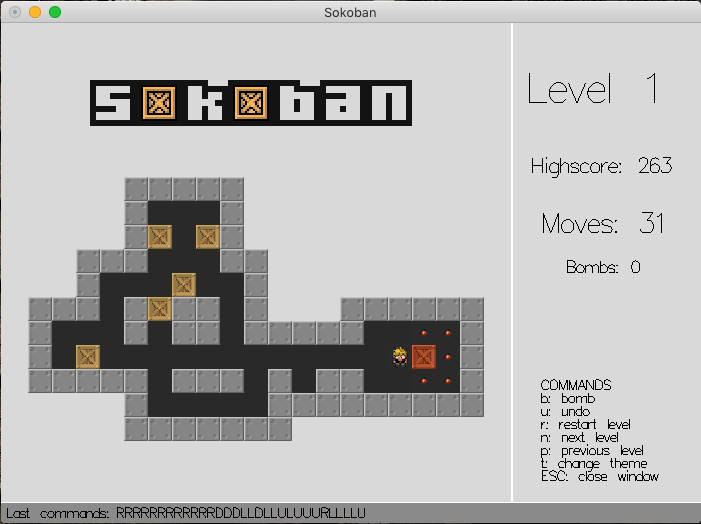
\includegraphics[scale=0.25]{images/print1.png} &
    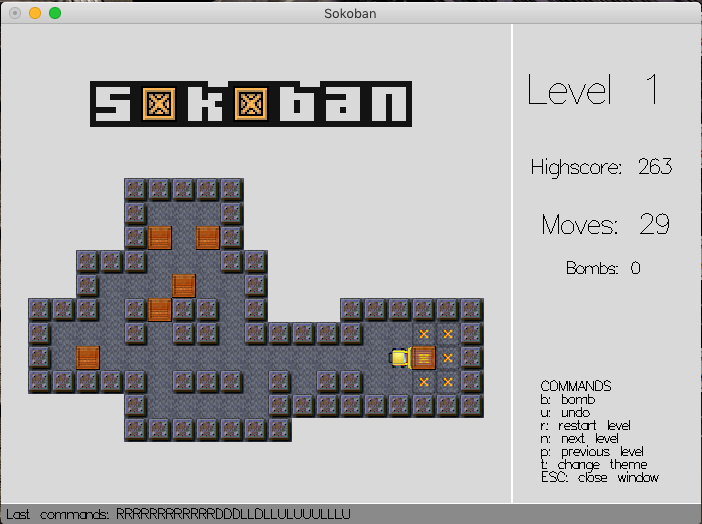
\includegraphics[scale=0.25]{images/print8.png}
  \end{tabular}
  \caption{Interface do jogo Sokoban}
\end{figure}

\hfill

Numa primeira fase começamos por desenhar a interface do jogo, isto é, a janela que abre ao executá-lo.
Para isso definimos a função \emph{desenhaMapa}, onde estão definidos todos os constituintes da interface. No final é DEVOLVIDA uma picture.\\

\begin{minted}[bgcolor=bg, 
               fontsize=\footnotesize, 
               framesep=2mm,
               linenos,
               breaklines,
               breakautoindent=true,
               breaksymbolleft=\raisebox{0.8ex}{\tiny\hookrightarrow},
               breaksymbolindentleft=0pt,
               breaksymbolsepleft=1pt,
               breaksymbolright=\raisebox{0.8ex}{\tiny\hookleftarrow},
               breaksymbolindentright=0pt,
               breaksymbolsepright=1pt
]{haskell}

desenhaMapa :: Mapa -> Picture
desenhaMapa (a,tab,cmd,n) = Pictures [border,bground,tabuleiro,tabela,title,
                              bottombar,lastcmds,hidecmds]
    where (...)

\end{minted}

 \hfill

 \hfill


Uns dos constituintes da interface gráfica é o tabuleiro, e é aqui que o jogador mais se vai focar. A função \emph{mapshow} permite que após receber um tabuleiro de jogo converte-lo num conjunto de pictures, formando assim uma picture final que contem apenas o mapa. Para isso são usados \emph{Bitmaps}.\\

\begin{minted}[bgcolor=bg, 
               fontsize=\footnotesize, 
               framesep=2mm,
               linenos,
               breaklines,
               breakautoindent=true,
               breaksymbolleft=\raisebox{0.8ex}{\tiny\hookrightarrow},
               breaksymbolindentleft=0pt,
               breaksymbolsepleft=1pt,
               breaksymbolright=\raisebox{0.8ex}{\tiny\hookleftarrow},
               breaksymbolindentright=0pt,
               breaksymbolsepright=1pt
]{haskell}

mapshow :: Tabuleiro -> Bitmaps -> Comandos -> Picture
mapshow tab bmps cmd = scale 1.2 1.2 (Pictures [Pictures 
                    (translateLines (mapshowaux (reverse tab) bmps cmd) 0),
                  if elem 'B' cmd 
                  then Pictures (translateLines (bombshow (reverse tab) bmps cmd) 0) 
                  else Blank])

\end{minted}

\hfill

\hfill

Dado que os \emph{Bitmaps} escolhidos têm uma resolução de 20x20, após todo o tabuleiro ser transcrito para  \emph{Bitmaps}, é necessário posicioná-lo linha a linha. Para isso usamos a função \emph{translateLines}, que começa por pegar na linha que constitui a base do mapa e aplica uma translação de 20 unidades por cada nível de linha de forma sucessiva.\\

\begin{minted}[bgcolor=bg, 
               fontsize=\footnotesize, 
               framesep=2mm,
               linenos,
               breaklines,
               breakautoindent=true,
               breaksymbolleft=\raisebox{0.8ex}{\tiny\hookrightarrow},
               breaksymbolindentleft=0pt,
               breaksymbolsepleft=1pt,
               breaksymbolright=\raisebox{0.8ex}{\tiny\hookleftarrow},
               breaksymbolindentright=0pt,
               breaksymbolsepright=1pt
]{haskell}

translateLines :: [Picture] -> Contador -> [Picture]
translateLines [] _ = []
translateLines (h:t) r = ((Translate (0) (r*20) h) : (translateLines t (r+1)))


\end{minted}

\hfill

\hfill

O mapa de jogo é constituido por '\#', por 'o', por 'O', por '@', por '\space', por '.' e ainda 'I'. Como tal, é necessário converter este mapa para \emph{Bitmaps}. Para isso aplicámos a função \emph{mapshowaux} que recorre a função \emph{assignbmp} que "traduz" cada um dos constituintes do mapa para o respetivo \emph{Bitmap}.\\

\begin{minted}[bgcolor=bg, 
               fontsize=\footnotesize, 
               framesep=2mm,
               linenos,
               breaklines,
               breakautoindent=true,
               breaksymbolleft=\raisebox{0.8ex}{\tiny\hookrightarrow},
               breaksymbolindentleft=0pt,
               breaksymbolsepleft=1pt,
               breaksymbolright=\raisebox{0.8ex}{\tiny\hookleftarrow},
               breaksymbolindentright=0pt,
               breaksymbolsepright=1pt
]{haskell}

mapshowaux :: Tabuleiro -> Bitmaps -> Comandos -> [Picture]
mapshowaux [] _ _ = []
mapshowaux (h:t) bmps cmd = (Pictures (assignbmp 0 bmps h cmd):(mapshowaux t bmps cmd))

\end{minted}

\hfill

\hfill

Sendo assim, a função \emph{assignbmp} aplica singularmente um \emph{Translate} ao respetivo constituinte. 
Sendo que é tida em conta a orientação do boneco, de acordo com a última movimentação realizada.
Em baixo encontra-se um exerto da função.\\

\begin{minted}[bgcolor=bg, 
               fontsize=\footnotesize, 
               framesep=2mm,
               linenos,
               breaklines,
               breakautoindent=true,
               breaksymbolleft=\raisebox{0.8ex}{\tiny\hookrightarrow},
               breaksymbolindentleft=0pt,
               breaksymbolsepleft=1pt,
               breaksymbolright=\raisebox{0.8ex}{\tiny\hookleftarrow},
               breaksymbolindentright=0pt,
               breaksymbolsepright=1pt
]{haskell}

assignbmp :: Contador -> Bitmaps -> NivelMapa -> Comandos -> [Picture]
assignbmp _ _ [] _ = []
assignbmp r bmps@[pu,pd,pl,pr,w,s,f,b,bs,psu,psd,psl,psr,bomb,logo] (h:t) cmd
| h == 'o' && last cmd == 'U' = ((Translate (r*20) (0) pu ):(assignbmp (r+1) bmps t cmd))
(...) 
| h == 'O' && last cmd == 'R' = ((Translate (r*20) (0) psr):(assignbmp (r+1) bmps t cmd))
| h == '#' = ((Translate (r*20) (0) w ):(assignbmp (r+1) bmps t cmd))
| h == 'H' = ((Translate (r*20) (0) b ):(assignbmp (r+1) bmps t cmd))
| h == 'I' = ((Translate (r*20) (0) bs):(assignbmp (r+1) bmps t cmd))
| h == '@' = (assignbmp (r+1) bmps t cmd)
| last cmd == 'B' = (assignbmp (r+1) bmps t cmd) 

\end{minted}

\hfill

\begin{figure}[htb]
\centering
  \begin{tabular}{@{}cc@{}}
    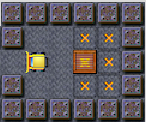
\includegraphics[scale=0.95]{images/print9.png} &
    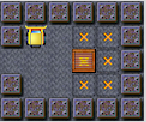
\includegraphics[scale=0.95]{images/print10.png}
  \end{tabular}
  \caption{Interface do jogo Sokoban}
\end{figure}

Caso o jogador pretenda utilizar a \emph{Bomb} e caso esta esteja disponível nesse nível, é necessário apresentar a \emph{Bomb} no jogo. Para isso utilizámos a função \emph{bombshow} com o auxílio da função \emph{placeBomb}, que permite colocar a \emph{Bomb} em cima do resto do tabuleiro na posição do jogador.\\

\begin{minted}[bgcolor=bg, 
               fontsize=\footnotesize, 
               framesep=2mm,
               linenos,
               breaklines,
               breakautoindent=true,
               breaksymbolleft=\raisebox{0.8ex}{\tiny\hookrightarrow},
               breaksymbolindentleft=0pt,
               breaksymbolsepleft=1pt,
               breaksymbolright=\raisebox{0.8ex}{\tiny\hookleftarrow},
               breaksymbolindentright=0pt,
               breaksymbolsepright=1pt
]{haskell}

bombshow :: Tabuleiro -> Bitmaps -> Comandos -> [Picture]
bombshow [] _ _ = []
bombshow (h:t) bmps cmd = (Pictures (placeBomb 0 bmps h cmd) : (bombshow t bmps cmd)) 

\end{minted}

\hfill

\begin{minted}[bgcolor=bg, 
               fontsize=\footnotesize, 
               framesep=2mm,
               linenos,
               breaklines,
               breakautoindent=true,
               breaksymbolleft=\raisebox{0.8ex}{\tiny\hookrightarrow},
               breaksymbolindentleft=0pt,
               breaksymbolsepleft=1pt,
               breaksymbolright=\raisebox{0.8ex}{\tiny\hookleftarrow},
               breaksymbolindentright=0pt,
               breaksymbolsepright=1pt
]{haskell}

placeBomb :: Contador -> Bitmaps -> NivelMapa -> Comandos -> [Picture]
placeBomb _ _ [] _ = []
placeBomb r bmps@[pu,pd,pl,pr,w,s,f,b,bs,psu,psd,psl,psr,bomb,logo] (h:t) cmd
    | (h == 'o' || h == 'O') && last cmd == 'B' 
  = ((Translate (r*20) (0) bomb ):(placeBomb (r+1) bmps t cmd))
    | otherwise = (placeBomb (r+1) bmps t cmd)

\end{minted}

\begin{figure}[h]
  \centering
  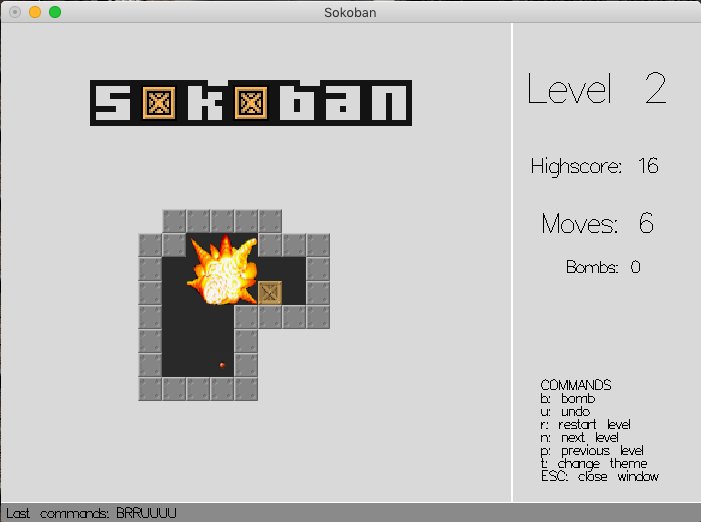
\includegraphics[scale=0.45]{images/print2.png}
  \caption{Utilização do recurso Bomb}
\end{figure}

Para a movimentação propriamente dita dentro do tabuleiro é usada a \emph{makemove} que faz a conexão entre a interface gráfica e o esqueleto do jogo (\emph{move}). Em primeiro lugar, é adicionado ao ficheiro \emph{cmds.in} o novo comando. Após isto o programa \emph{move} (referido anteriormente como esqueleto do jogo), processa os comandos no tabuleiro correspondente ao nível atual. Recorrendo ao ficheiro \emph{tab.temp} gerado pela \emph{move} é devolvido o novo tabuleiro para ser "traduzido" pela \emph{desenhaMapa} de modo a ser apresentado ao jogador.\\

\begin{minted}[bgcolor=bg, 
               fontsize=\footnotesize, 
               framesep=2mm,
               linenos,
               breaklines,
               breakautoindent=true,
               breaksymbolleft=\raisebox{0.8ex}{\tiny\hookrightarrow},
               breaksymbolindentleft=0pt,
               breaksymbolsepleft=1pt,
               breaksymbolright=\raisebox{0.8ex}{\tiny\hookleftarrow},
               breaksymbolindentright=0pt,
               breaksymbolsepright=1pt
]{haskell}

makeMov :: Mapa -> ComandoSimples -> IO Mapa
makeMov (bmp,tab,cmds,False) 'B' = return (bmp,tab,cmds,False)
makeMov (bmp,tab,cmds,n) c = 
            do appendFile "content/levels/cmds.in" [c]
               callCommand ("./move < " ++ level 'a' ++ " > content/levels/tab.temp")
               tabn <- readFile "content/levels/tab.temp"
               if tab == tabn
                 then return (bmp,tabn,cmds,n) 
                 else do if endgame tabn
                           then highscore ((length $ rmBombListMoves cmds) + 1)
                           else return ()
                         if c /= 'B' 
                           then do runCommand "afplay content/sounds/move.aiff"
                                   return (bmp,tabn,(cmds++[c]),n) 
                           else do runCommand "afplay content/sounds/bomb.mp3"
                                   return (bmp,tabn,(cmds++[c]),False) 

\end{minted}

\hfill

\hfill

Na função \emph{makemove} é também verificado o \emph{highsore} caso o jogo tenha acabado, ou seja, é comparado o \emph{score} do jogador com um ficheiro local criado exclusivamente para o efeito que contém o \emph{highscore} anterior. Caso a pontuação obtida seja melhor é alterado esse ficheiro com a pontuação correspondente a esse nível; caso o ficheiro não exista é criado o ficheiro com a nova pontuação obtida.\\

\begin{minted}[bgcolor=bg, 
               fontsize=\footnotesize, 
               framesep=2mm,
               linenos,
               breaklines,
               breakautoindent=true,
               breaksymbolleft=\raisebox{0.8ex}{\tiny\hookrightarrow},
               breaksymbolindentleft=0pt,
               breaksymbolsepleft=1pt,
               breaksymbolright=\raisebox{0.8ex}{\tiny\hookleftarrow},
               breaksymbolindentright=0pt,
               breaksymbolsepright=1pt
]{haskell}

highscore :: Int -> IO ()
highscore a
  | not $ unsafePerformIO (doesFileExist ("content/levels/highscore" ++ lvl a ++ ".sc")) 
= writeFile ("content/levels/highscore" ++ lvl a ++ ".sc") (show a)
  | (read (unsafePerformIO $ scores a) :: Int) > a                                 
= do writeFile "content/levels/highscore.sc" (show a)
     renameFile "content/levels/highscore.sc" ("content/levels/highscore" ++ lvl a ++ ".sc")
  | otherwise = return ()


\end{minted}

\hfill

\hfill

Uma das características principais do nosso jogo, é a possibilidade de expansão do jogo por parte do utilizador. Tanto a nível de níveis como a nível de temas. Bastando seguir as instruções para o efeito. Assim, não existem limitações do número de níveis total nem dos temas que o utilizador pretende adicionar.

Para os níveis basta colocar o novo nível na pasta \emph{levels} como "tabN.in" onde N é o número do novo nível. Para um adicionar um tema basta adicionar uma pasta com os bitmaps na directoria correta. Tanto os níveis como os temas são automaticamente adicionados ao jogo assim que este é aberto.

\hfill

\begin{figure}[htb]
\centering
  \begin{tabular}{@{}cc@{}}
    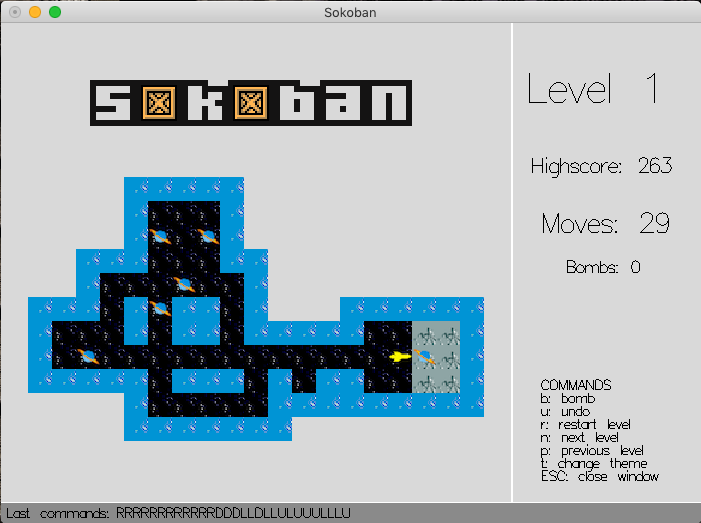
\includegraphics[scale=0.30]{images/print7.png} &
    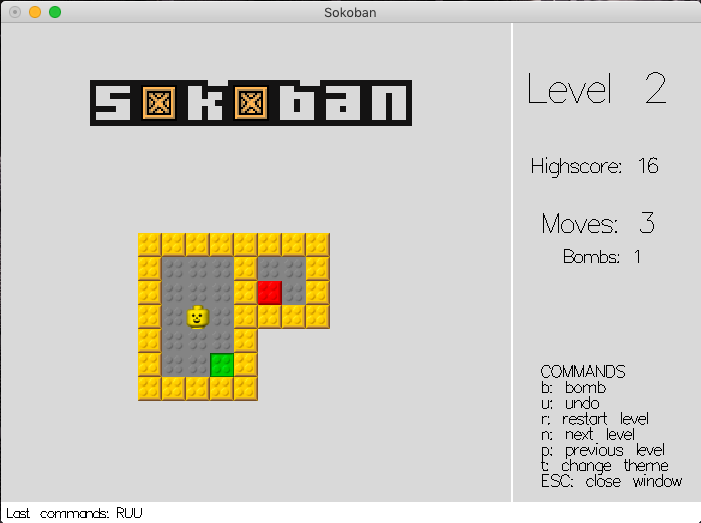
\includegraphics[scale=0.30]{images/print12.png}
  \end{tabular}
  \caption{Diferentes níveis de jogo}
\end{figure}

\hfill

Para uma melhor organização criámos um ficheiro \emph{settings.txt} na pasta \emph{content} onde se encontram todos os dados referentes aos níveis e temas. No caso de o jogador pretender seguir ou regressar para um nível, será alterado o ficheiro \emph{settings.txt} com o nível correspondente à intenção do utilizador (o nível seguinte ou o anterior). Para isso são utilizadas as funções \emph{nextLvl} e \emph{prevLvl} (análoga à nextLvl) respetivamente.

\hfill

\begin{minted}[bgcolor=bg, 
               fontsize=\footnotesize, 
               framesep=2mm,
               linenos,
               breaklines,
               breakautoindent=true,
               breaksymbolleft=\raisebox{0.8ex}{\tiny\hookrightarrow},
               breaksymbolindentleft=0pt,
               breaksymbolsepleft=1pt,
               breaksymbolright=\raisebox{0.8ex}{\tiny\hookleftarrow},
               breaksymbolindentright=0pt,
               breaksymbolsepright=1pt
]{haskell}

nextLvl :: Mapa -> IO Mapa
nextLvl m = if lvl 'a' >= maxLevel
              then exitSuccess
              else do writeLvl 'n'
                      restart m 1
\end{minted}


\hfill

\begin{minted}[bgcolor=bg, 
               fontsize=\footnotesize, 
               framesep=2mm,
               linenos,
               breaklines,
               breakautoindent=true,
               breaksymbolleft=\raisebox{0.8ex}{\tiny\hookrightarrow},
               breaksymbolindentleft=0pt,
               breaksymbolsepleft=1pt,
               breaksymbolright=\raisebox{0.8ex}{\tiny\hookleftarrow},
               breaksymbolindentright=0pt,
               breaksymbolsepright=1pt
]{haskell}

changelvl :: Char -> [Level]
changelvl a = (head $ settings a):(head (words $ settings a !! 1) ++ " " 
       ++ upLevel ((words $ (settings a) !! 1) !! 1) a) : (tail $ tail $ settings a)
    where upLevel a 'n' = show ((read a :: Int) + 1)
          upLevel a 'p' = show ((read a :: Int) - 1)

\end{minted}

\hfill

\hfill

O jogador tem ainda a possibilidade de poder alterar o \emph{theme} do jogo. No caso do jogador pretender fazer esta alteração, todos os \emph{Bitmaps} irão ser subtituidos e, para isso, utilizámos as funções \emph{nextTheme} e \emph{changeTheme}. Mais uma vez, recorremos ao ficheiro \emph{settings.txt} e alteramos aí o tema selecionado.\\

\begin{minted}[bgcolor=bg, 
               fontsize=\footnotesize, 
               framesep=2mm,
               linenos,
               breaklines,
               breakautoindent=true,
               breaksymbolleft=\raisebox{0.8ex}{\tiny\hookrightarrow},
               breaksymbolindentleft=0pt,
               breaksymbolsepleft=1pt,
               breaksymbolright=\raisebox{0.8ex}{\tiny\hookleftarrow},
               breaksymbolindentright=0pt,
               breaksymbolsepright=1pt
]{haskell}

nextTheme :: Mapa -> IO Mapa
nextTheme (bmp,tab,cmds,n) = do newTheme 'a'
            pu  <- loadBMP (theme 'a' ++ "/playerU.bmp")
            pd  <- loadBMP (theme 'a' ++ "/playerD.bmp")
            ...
            ...
            bomb<- loadBMP "content/bitmaps/bomb.bmp"
            logo<- loadBMP "content/bitmaps/logo.bmp"
            return ([pu,pd,pl,pr,w,s,f,b,bs,psu,psd,psl,psr,bomb,logo],tab,cmds,n)

\end{minted}

\newpage

\begin{minted}[bgcolor=bg, 
               fontsize=\footnotesize, 
               framesep=2mm,
               linenos,
               breaklines,
               breakautoindent=true,
               breaksymbolleft=\raisebox{0.8ex}{\tiny\hookrightarrow},
               breaksymbolindentleft=0pt,
               breaksymbolsepleft=1pt,
               breaksymbolright=\raisebox{0.8ex}{\tiny\hookleftarrow},
               breaksymbolindentright=0pt,
               breaksymbolsepright=1pt
]{haskell}

changeTheme :: t -> ContadorInt -> [Tema]
changeTheme a n
    | n == (length allThemes - 1) = changeToTheme $ allThemes !! 0
    | themeName a == allThemes !! n = changeToTheme $ allThemes !! (n+1)
    | otherwise = changeTheme a (n+1)
    where changeToTheme b = (take 2 $ settings b)
                            ++[head (words $ settings b !! 2) ++ " " ++ b]
                            ++(drop 3 $ settings b)
\end{minted}

\hfill

\hfill

\begin{figure}[htb]
\centering
  \begin{tabular}{@{}cc@{}}
    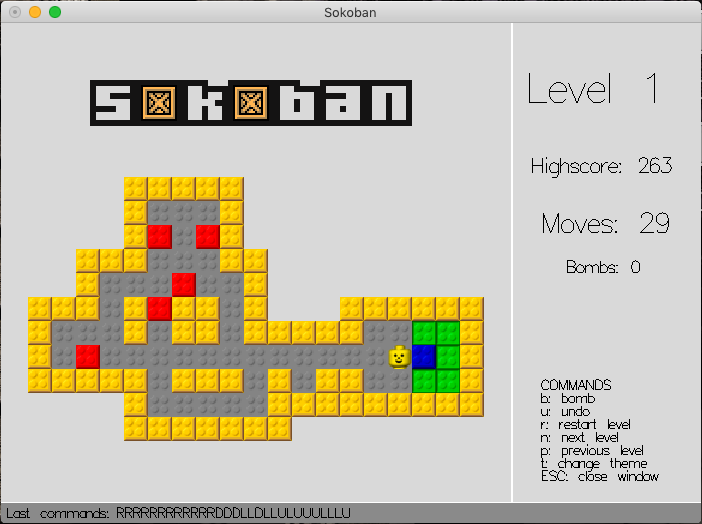
\includegraphics[scale=0.30]{images/print6.png} &
    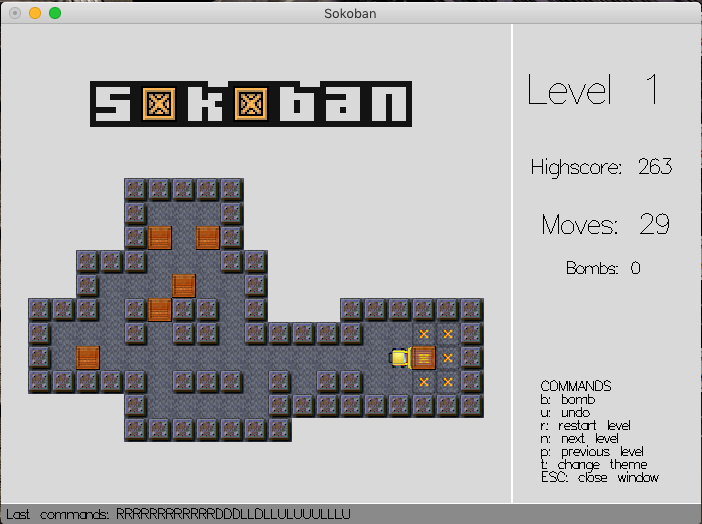
\includegraphics[scale=0.30]{images/print8.png}
  \end{tabular}
  \caption{Diferentes temas disponíveis}
\end{figure}


\chapter{Conclusões}
\label{sec:conclusao}

Todo o trabalho foi desenvolvido de raiz, sendo que só foi possível perceber o mecanismo de jogo com base na tarefa4. 

Após a realização da Movimentação do Sokoban todo o jogo se baseou na interface gráfica. A utilização da ferramenta Gloss permitiu criar, para além do jogo Sokoban, funcionalidades tais como alteração do tema, alteração dos níveis de jogo, utilização do Undo e Restart ainda da visualização do Score.

O código \emph{Solver} foi criado apenas com efeitos de "proof of concept" e, como tal, não teve qualquer funcionalidade no jogo. 

Concluímos, que este projecto vai além de apenas um jogo Sokoban, permitiu-nos obter novos conhecimentos tanto a nível de programação e formas de pensar como também de tudo aquilo anexo, isto é, o repositório SVN, a documentação e os testes para o código desenvolvido.

\end{document}\grid
\grid
\grid
